\documentclass[1p]{elsarticle_modified}
%\bibliographystyle{elsarticle-num}

%\usepackage[colorlinks]{hyperref}
%\usepackage{abbrmath_seonhwa} %\Abb, \Ascr, \Acal ,\Abf, \Afrak
\usepackage{amsfonts}
\usepackage{amssymb}
\usepackage{amsmath}
\usepackage{amsthm}
\usepackage{scalefnt}
\usepackage{amsbsy}
\usepackage{kotex}
\usepackage{caption}
\usepackage{subfig}
\usepackage{color}
\usepackage{graphicx}
\usepackage{xcolor} %% white, black, red, green, blue, cyan, magenta, yellow
\usepackage{float}
\usepackage{setspace}
\usepackage{hyperref}

\usepackage{tikz}
\usetikzlibrary{arrows}

\usepackage{multirow}
\usepackage{array} % fixed length table
\usepackage{hhline}

%%%%%%%%%%%%%%%%%%%%%
\makeatletter
\renewcommand*\env@matrix[1][\arraystretch]{%
	\edef\arraystretch{#1}%
	\hskip -\arraycolsep
	\let\@ifnextchar\new@ifnextchar
	\array{*\c@MaxMatrixCols c}}
\makeatother %https://tex.stackexchange.com/questions/14071/how-can-i-increase-the-line-spacing-in-a-matrix
%%%%%%%%%%%%%%%

\usepackage[normalem]{ulem}

\newcommand{\msout}[1]{\ifmmode\text{\sout{\ensuremath{#1}}}\else\sout{#1}\fi}
%SOURCE: \msout is \stkout macro in https://tex.stackexchange.com/questions/20609/strikeout-in-math-mode

\newcommand{\cancel}[1]{
	\ifmmode
	{\color{red}\msout{#1}}
	\else
	{\color{red}\sout{#1}}
	\fi
}

\newcommand{\add}[1]{
	{\color{blue}\uwave{#1}}
}

\newcommand{\replace}[2]{
	\ifmmode
	{\color{red}\msout{#1}}{\color{blue}\uwave{#2}}
	\else
	{\color{red}\sout{#1}}{\color{blue}\uwave{#2}}
	\fi
}

\newcommand{\Sol}{\mathcal{S}} %segment
\newcommand{\D}{D} %diagram
\newcommand{\A}{\mathcal{A}} %arc


%%%%%%%%%%%%%%%%%%%%%%%%%%%%%5 test

\def\sl{\operatorname{\textup{SL}}(2,\Cbb)}
\def\psl{\operatorname{\textup{PSL}}(2,\Cbb)}
\def\quan{\mkern 1mu \triangleright \mkern 1mu}

\theoremstyle{definition}
\newtheorem{thm}{Theorem}[section]
\newtheorem{prop}[thm]{Proposition}
\newtheorem{lem}[thm]{Lemma}
\newtheorem{ques}[thm]{Question}
\newtheorem{cor}[thm]{Corollary}
\newtheorem{defn}[thm]{Definition}
\newtheorem{exam}[thm]{Example}
\newtheorem{rmk}[thm]{Remark}
\newtheorem{alg}[thm]{Algorithm}

\newcommand{\I}{\sqrt{-1}}
\begin{document}

%\begin{frontmatter}
%
%\title{Boundary parabolic representations of knots up to 8 crossings}
%
%%% Group authors per affiliation:
%\author{Yunhi Cho} 
%\address{Department of Mathematics, University of Seoul, Seoul, Korea}
%\ead{yhcho@uos.ac.kr}
%
%
%\author{Seonhwa Kim} %\fnref{s_kim}}
%\address{Center for Geometry and Physics, Institute for Basic Science, Pohang, 37673, Korea}
%\ead{ryeona17@ibs.re.kr}
%
%\author{Hyuk Kim}
%\address{Department of Mathematical Sciences, Seoul National University, Seoul 08826, Korea}
%\ead{hyukkim@snu.ac.kr}
%
%\author{Seokbeom Yoon}
%\address{Department of Mathematical Sciences, Seoul National University, Seoul, 08826,  Korea}
%\ead{sbyoon15@snu.ac.kr}
%
%\begin{abstract}
%We find all boundary parabolic representation of knots up to 8 crossings.
%
%\end{abstract}
%\begin{keyword}
%    \MSC[2010] 57M25 
%\end{keyword}
%
%\end{frontmatter}

%\linenumbers
%\tableofcontents
%
\newcommand\colored[1]{\textcolor{white}{\rule[-0.35ex]{0.8em}{1.4ex}}\kern-0.8em\color{red} #1}%
%\newcommand\colored[1]{\textcolor{white}{ #1}\kern-2.17ex	\textcolor{white}{ #1}\kern-1.81ex	\textcolor{white}{ #1}\kern-2.15ex\color{red}#1	}

{\Large $\underline{12n_{0601}~(K12n_{0601})}$}

\setlength{\tabcolsep}{10pt}
\renewcommand{\arraystretch}{1.6}
\vspace{1cm}\begin{tabular}{m{100pt}>{\centering\arraybackslash}m{274pt}}
\multirow{5}{120pt}{
	\centering
	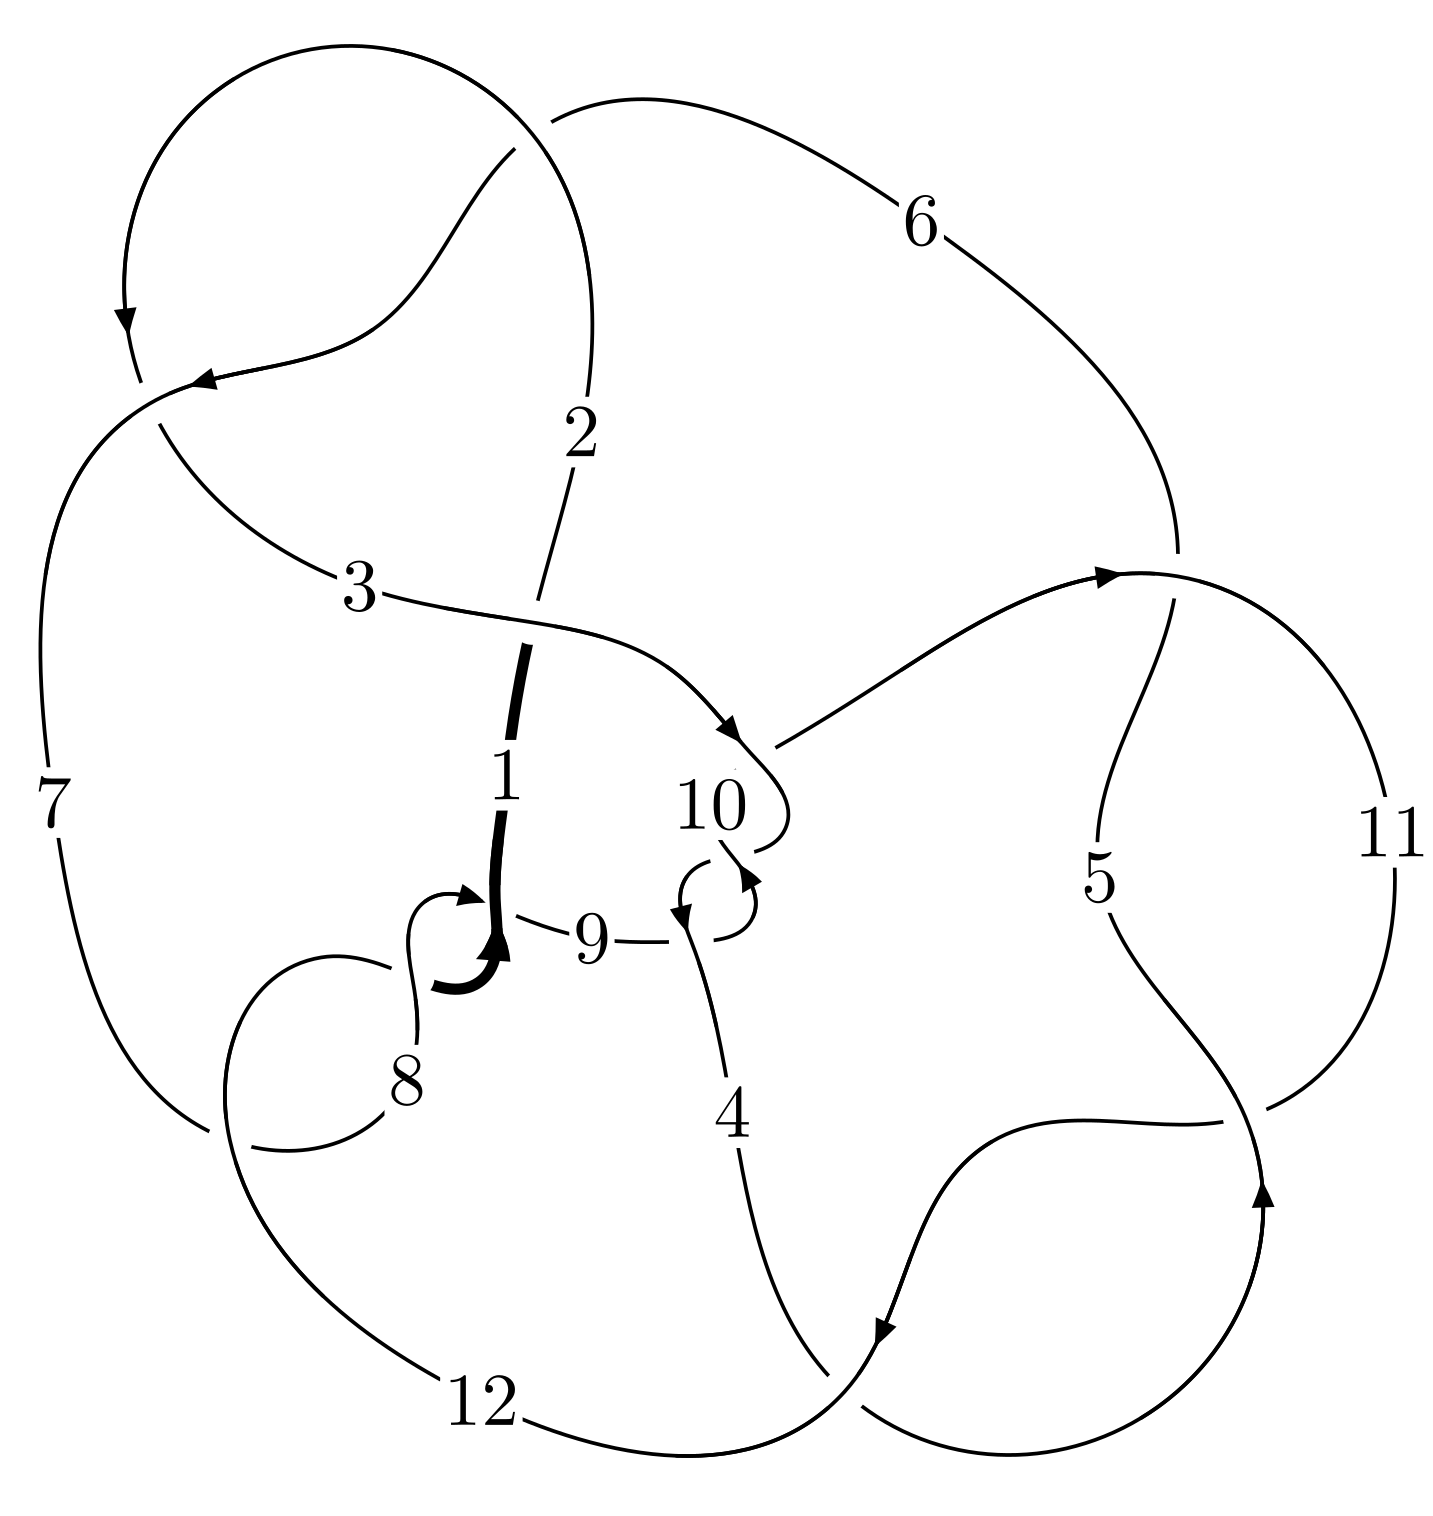
\includegraphics[width=112pt]{../../../GIT/diagram.site/Diagrams/png/2690_12n_0601.png}\\
\ \ \ A knot diagram\footnotemark}&
\allowdisplaybreaks
\textbf{Linearized knot diagam} \\
\cline{2-2}
 &
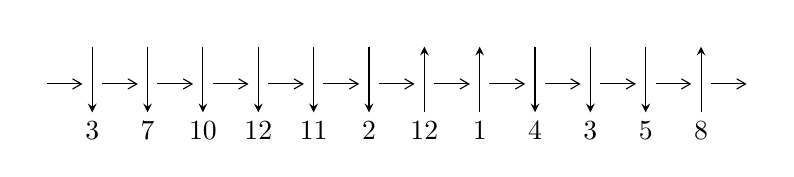
\begin{tikzpicture}[x=20pt, y=17pt]
	% nodes
	\node (C0) at (0, 0) {};
	\node (C1) at (1, 0) {};
	\node (C1U) at (1, +1) {};
	\node (C1D) at (1, -1) {3};

	\node (C2) at (2, 0) {};
	\node (C2U) at (2, +1) {};
	\node (C2D) at (2, -1) {7};

	\node (C3) at (3, 0) {};
	\node (C3U) at (3, +1) {};
	\node (C3D) at (3, -1) {10};

	\node (C4) at (4, 0) {};
	\node (C4U) at (4, +1) {};
	\node (C4D) at (4, -1) {12};

	\node (C5) at (5, 0) {};
	\node (C5U) at (5, +1) {};
	\node (C5D) at (5, -1) {11};

	\node (C6) at (6, 0) {};
	\node (C6U) at (6, +1) {};
	\node (C6D) at (6, -1) {2};

	\node (C7) at (7, 0) {};
	\node (C7U) at (7, +1) {};
	\node (C7D) at (7, -1) {12};

	\node (C8) at (8, 0) {};
	\node (C8U) at (8, +1) {};
	\node (C8D) at (8, -1) {1};

	\node (C9) at (9, 0) {};
	\node (C9U) at (9, +1) {};
	\node (C9D) at (9, -1) {4};

	\node (C10) at (10, 0) {};
	\node (C10U) at (10, +1) {};
	\node (C10D) at (10, -1) {3};

	\node (C11) at (11, 0) {};
	\node (C11U) at (11, +1) {};
	\node (C11D) at (11, -1) {5};

	\node (C12) at (12, 0) {};
	\node (C12U) at (12, +1) {};
	\node (C12D) at (12, -1) {8};
	\node (C13) at (13, 0) {};

	% arrows
	\draw[->,>={angle 60}]
	(C0) edge (C1) (C1) edge (C2) (C2) edge (C3) (C3) edge (C4) (C4) edge (C5) (C5) edge (C6) (C6) edge (C7) (C7) edge (C8) (C8) edge (C9) (C9) edge (C10) (C10) edge (C11) (C11) edge (C12) (C12) edge (C13) ;	\draw[->,>=stealth]
	(C1U) edge (C1D) (C2U) edge (C2D) (C3U) edge (C3D) (C4U) edge (C4D) (C5U) edge (C5D) (C6U) edge (C6D) (C7D) edge (C7U) (C8D) edge (C8U) (C9U) edge (C9D) (C10U) edge (C10D) (C11U) edge (C11D) (C12D) edge (C12U) ;
	\end{tikzpicture} \\
\hhline{~~} \\& 
\textbf{Solving Sequence} \\ \cline{2-2} 
 &
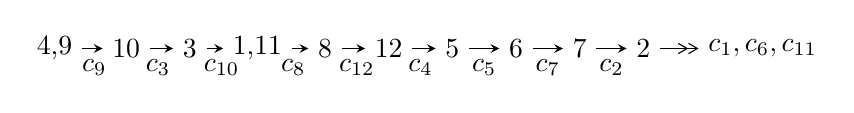
\begin{tikzpicture}[x=23pt, y=7pt]
	% node
	\node (A0) at (-1/8, 0) {4,9};
	\node (A1) at (1, 0) {10};
	\node (A2) at (2, 0) {3};
	\node (A3) at (49/16, 0) {1,11};
	\node (A4) at (33/8, 0) {8};
	\node (A5) at (41/8, 0) {12};
	\node (A6) at (49/8, 0) {5};
	\node (A7) at (57/8, 0) {6};
	\node (A8) at (65/8, 0) {7};
	\node (A9) at (73/8, 0) {2};
	\node (C1) at (1/2, -1) {$c_{9}$};
	\node (C2) at (3/2, -1) {$c_{3}$};
	\node (C3) at (5/2, -1) {$c_{10}$};
	\node (C4) at (29/8, -1) {$c_{8}$};
	\node (C5) at (37/8, -1) {$c_{12}$};
	\node (C6) at (45/8, -1) {$c_{4}$};
	\node (C7) at (53/8, -1) {$c_{5}$};
	\node (C8) at (61/8, -1) {$c_{7}$};
	\node (C9) at (69/8, -1) {$c_{2}$};
	\node (A10) at (11, 0) {$c_{1},c_{6},c_{11}$};

	% edge
	\draw[->,>=stealth]	
	(A0) edge (A1) (A1) edge (A2) (A2) edge (A3) (A3) edge (A4) (A4) edge (A5) (A5) edge (A6) (A6) edge (A7) (A7) edge (A8) (A8) edge (A9) ;
	\draw[->>,>={angle 60}]	
	(A9) edge (A10);
\end{tikzpicture} \\ 

\end{tabular} \\

\footnotetext{
The image of knot diagram is generated by the software ``\textbf{Draw programme}" developed by Andrew Bartholomew(\url{http://www.layer8.co.uk/maths/draw/index.htm\#Running-draw}), where we modified some parts for our purpose(\url{https://github.com/CATsTAILs/LinksPainter}).
}\phantom \\ \newline 
\centering \textbf{Ideals for irreducible components\footnotemark of $X_{\text{par}}$} 
 
\begin{align*}
I^u_{1}&=\langle 
u^{12}- u^{11}-3 u^{10}-18 u^9-28 u^8-82 u^7-102 u^6-220 u^5-203 u^4-209 u^3+9 u^2+16 b-46 u+22,\\
\phantom{I^u_{1}}&\phantom{= \langle  }-3 u^{12}-2 u^{11}-7 u^{10}+6 u^9-6 u^8+54 u^7+28 u^6+198 u^5+151 u^4+188 u^3-133 u^2+32 a+12 u-54,\\
\phantom{I^u_{1}}&\phantom{= \langle  }u^{13}+3 u^{12}+9 u^{11}+17 u^{10}+36 u^9+52 u^8+86 u^7+86 u^6+81 u^5+27 u^4+25 u^3-7 u^2+2 u-2\rangle \\
I^u_{2}&=\langle 
-5 u^9+25 u^8-15 u^7+23 u^6-165 u^5+221 u^4-167 u^3+423 u^2+144 b-112 u+44,\\
\phantom{I^u_{2}}&\phantom{= \langle  }73 u^9-23 u^8+3 u^7-433 u^6+465 u^5-307 u^4+1531 u^3+63 u^2+288 a+584 u-52,\\
\phantom{I^u_{2}}&\phantom{= \langle  }u^{10}- u^9+u^8-7 u^7+11 u^6-13 u^5+33 u^4-23 u^3+26 u^2-20 u+8\rangle \\
I^u_{3}&=\langle 
a^3 u+a^3- a^2 u+2 a^2-3 a u+b-3 a- u-3,\;2 a^4-3 a^3 u+a^3-6 a^2+3 a u-5 a+u-1,\;u^2+1\rangle \\
I^u_{4}&=\langle 
b+1,\;6 a- u-3,\;u^2+3\rangle \\
I^u_{5}&=\langle 
2 a^2+b-2 a+2,\;2 a^3-2 a^2+3 a-1,\;u-1\rangle \\
\\
I^v_{1}&=\langle 
a,\;b+1,\;v-1\rangle \\
\end{align*}
\raggedright * 6 irreducible components of $\dim_{\mathbb{C}}=0$, with total 37 representations.\\
\footnotetext{All coefficients of polynomials are rational numbers. But the coefficients are sometimes approximated in decimal forms when there is not enough margin.}
\newpage
\renewcommand{\arraystretch}{1}
\centering \section*{I. $I^u_{1}= \langle u^{12}- u^{11}+\cdots+16 b+22,\;-3 u^{12}-2 u^{11}+\cdots+32 a-54,\;u^{13}+3 u^{12}+\cdots+2 u-2 \rangle$}
\flushleft \textbf{(i) Arc colorings}\\
\begin{tabular}{m{7pt} m{180pt} m{7pt} m{180pt} }
\flushright $a_{4}=$&$\begin{pmatrix}0\\u\end{pmatrix}$ \\
\flushright $a_{9}=$&$\begin{pmatrix}1\\0\end{pmatrix}$ \\
\flushright $a_{10}=$&$\begin{pmatrix}1\\u^2\end{pmatrix}$ \\
\flushright $a_{3}=$&$\begin{pmatrix}u\\u^3+u\end{pmatrix}$ \\
\flushright $a_{1}=$&$\begin{pmatrix}\frac{3}{32} u^{12}+\frac{1}{16} u^{11}+\cdots-\frac{3}{8} u+\frac{27}{16}\\-0.0625000 u^{12}+0.0625000 u^{11}+\cdots+2.87500 u-1.37500\end{pmatrix}$ \\
\flushright $a_{11}=$&$\begin{pmatrix}u^2+1\\u^4+2 u^2\end{pmatrix}$ \\
\flushright $a_{8}=$&$\begin{pmatrix}\frac{3}{32} u^{12}+\frac{1}{16} u^{11}+\cdots-\frac{3}{8} u+\frac{27}{16}\\\frac{3}{16} u^{12}+\frac{3}{4} u^{11}+\cdots-\frac{1}{2} u-\frac{5}{8}\end{pmatrix}$ \\
\flushright $a_{12}=$&$\begin{pmatrix}1\\-\frac{1}{8} u^{11}-\frac{3}{8} u^{10}+\cdots-\frac{1}{4} u+\frac{1}{4}\end{pmatrix}$ \\
\flushright $a_{5}=$&$\begin{pmatrix}- u\\\frac{1}{8} u^{12}+\frac{3}{8} u^{11}+\cdots+\frac{1}{4} u^2+\frac{3}{4} u\end{pmatrix}$ \\
\flushright $a_{6}=$&$\begin{pmatrix}- u^3-2 u\\\frac{1}{8} u^{12}+\frac{3}{8} u^{11}+\cdots+\frac{1}{4} u^2+\frac{3}{4} u\end{pmatrix}$ \\
\flushright $a_{7}=$&$\begin{pmatrix}\frac{1}{32} u^{12}+\frac{1}{8} u^{11}+\cdots+\frac{5}{2} u+\frac{5}{16}\\\frac{1}{8} u^{12}+\frac{1}{8} u^{11}+\cdots-3 u+\frac{13}{8}\end{pmatrix}$ \\
\flushright $a_{2}=$&$\begin{pmatrix}\frac{3}{32} u^{12}+\frac{1}{4} u^{11}+\cdots+\frac{3}{4} u+\frac{15}{16}\\-\frac{1}{8} u^{12}+\frac{1}{16} u^{11}+\cdots+\frac{29}{8} u-\frac{7}{4}\end{pmatrix}$\\&\end{tabular}
\flushleft \textbf{(ii) Obstruction class $= -1$}\\~\\
\flushleft \textbf{(iii) Cusp Shapes $= -\frac{17}{8} u^{12}-\frac{27}{4} u^{11}-\frac{159}{8} u^{10}-\frac{153}{4} u^9-\frac{317}{4} u^8-\frac{469}{4} u^7-\frac{377}{2} u^6-\frac{781}{4} u^5-\frac{1383}{8} u^4-58 u^3-\frac{309}{8} u^2+\frac{9}{2} u-\frac{15}{4}$}\\~\\
\newpage\renewcommand{\arraystretch}{1}
\flushleft \textbf{(iv) u-Polynomials at the component}\newline \\
\begin{tabular}{m{50pt}|m{274pt}}
Crossings & \hspace{64pt}u-Polynomials at each crossing \\
\hline $$\begin{aligned}c_{1}\end{aligned}$$&$\begin{aligned}
&u^{13}+10 u^{12}+\cdots+651 u+169
\end{aligned}$\\
\hline $$\begin{aligned}c_{2},c_{6}\end{aligned}$$&$\begin{aligned}
&u^{13}-6 u^{12}+\cdots-27 u+13
\end{aligned}$\\
\hline $$\begin{aligned}c_{3},c_{4},c_{5}\\c_{9},c_{10},c_{11}\end{aligned}$$&$\begin{aligned}
&u^{13}-3 u^{12}+\cdots+2 u+2
\end{aligned}$\\
\hline $$\begin{aligned}c_{7},c_{8},c_{12}\end{aligned}$$&$\begin{aligned}
&u^{13}+6 u^{12}+\cdots+33 u+13
\end{aligned}$\\
\hline
\end{tabular}\\~\\
\newpage\renewcommand{\arraystretch}{1}
\flushleft \textbf{(v) Riley Polynomials at the component}\newline \\
\begin{tabular}{m{50pt}|m{274pt}}
Crossings & \hspace{64pt}Riley Polynomials at each crossing \\
\hline $$\begin{aligned}c_{1}\end{aligned}$$&$\begin{aligned}
&y^{13}-10 y^{12}+\cdots-63933 y-28561
\end{aligned}$\\
\hline $$\begin{aligned}c_{2},c_{6}\end{aligned}$$&$\begin{aligned}
&y^{13}-10 y^{12}+\cdots+651 y-169
\end{aligned}$\\
\hline $$\begin{aligned}c_{3},c_{4},c_{5}\\c_{9},c_{10},c_{11}\end{aligned}$$&$\begin{aligned}
&y^{13}+9 y^{12}+\cdots-24 y-4
\end{aligned}$\\
\hline $$\begin{aligned}c_{7},c_{8},c_{12}\end{aligned}$$&$\begin{aligned}
&y^{13}-10 y^{12}+\cdots+1531 y-169
\end{aligned}$\\
\hline
\end{tabular}\\~\\
\newpage\flushleft \textbf{(vi) Complex Volumes and Cusp Shapes}
$$\begin{array}{c|c|c}  
\text{Solutions to }I^u_{1}& \I (\text{vol} + \sqrt{-1}CS) & \text{Cusp shape}\\
 \hline 
\begin{aligned}
u &= -0.052333 + 0.714648 I \\
a &= -1.60779 + 0.26845 I \\
b &= \phantom{-}1.60510 + 0.10103 I\end{aligned}
 & \phantom{-}8.97858 + 3.36382 I & -4.98253 - 3.88513 I \\ \hline\begin{aligned}
u &= -0.052333 - 0.714648 I \\
a &= -1.60779 - 0.26845 I \\
b &= \phantom{-}1.60510 - 0.10103 I\end{aligned}
 & \phantom{-}8.97858 - 3.36382 I & -4.98253 + 3.88513 I \\ \hline\begin{aligned}
u &= -0.962101 + 0.964907 I \\
a &= -0.415380 + 1.110690 I \\
b &= \phantom{-}1.29540 + 0.78987 I\end{aligned}
 & \phantom{-}0.19846 + 6.55527 I & -1.94504 - 5.19831 I \\ \hline\begin{aligned}
u &= -0.962101 - 0.964907 I \\
a &= -0.415380 - 1.110690 I \\
b &= \phantom{-}1.29540 - 0.78987 I\end{aligned}
 & \phantom{-}0.19846 - 6.55527 I & -1.94504 + 5.19831 I \\ \hline\begin{aligned}
u &= -0.024468 + 0.460540 I \\
a &= \phantom{-}0.557073 + 0.142637 I \\
b &= -0.684651 + 0.431349 I\end{aligned}
 & \phantom{-}1.04755 - 1.45507 I & -1.76075 + 3.94050 I \\ \hline\begin{aligned}
u &= -0.024468 - 0.460540 I \\
a &= \phantom{-}0.557073 - 0.142637 I \\
b &= -0.684651 - 0.431349 I\end{aligned}
 & \phantom{-}1.04755 + 1.45507 I & -1.76075 - 3.94050 I \\ \hline\begin{aligned}
u &= \phantom{-}0.351244\phantom{ +0.000000I} \\
a &= \phantom{-}1.70634\phantom{ +0.000000I} \\
b &= \phantom{-}0.413951\phantom{ +0.000000I}\end{aligned}
 & -0.867716\phantom{ +0.000000I} & -13.5770\phantom{ +0.000000I} \\ \hline\begin{aligned}
u &= -0.19008 + 1.69584 I \\
a &= \phantom{-}0.448130 + 0.064643 I \\
b &= -1.186010 + 0.315331 I\end{aligned}
 & \phantom{-}13.21680 - 1.39421 I & \phantom{-}0.43458 + 4.61417 I \\ \hline\begin{aligned}
u &= -0.19008 - 1.69584 I \\
a &= \phantom{-}0.448130 - 0.064643 I \\
b &= -1.186010 - 0.315331 I\end{aligned}
 & \phantom{-}13.21680 + 1.39421 I & \phantom{-}0.43458 - 4.61417 I \\ \hline\begin{aligned}
u &= \phantom{-}0.89659 + 1.48771 I \\
a &= -0.615979 - 1.008550 I \\
b &= \phantom{-}1.44106 - 0.72214 I\end{aligned}
 & -5.5396 - 13.0547 I & -2.53712 + 6.01217 I\\
 \hline 
 \end{array}$$\newpage$$\begin{array}{c|c|c}  
\text{Solutions to }I^u_{1}& \I (\text{vol} + \sqrt{-1}CS) & \text{Cusp shape}\\
 \hline 
\begin{aligned}
u &= \phantom{-}0.89659 - 1.48771 I \\
a &= -0.615979 + 1.008550 I \\
b &= \phantom{-}1.44106 + 0.72214 I\end{aligned}
 & -5.5396 + 13.0547 I & -2.53712 - 6.01217 I \\ \hline\begin{aligned}
u &= -1.34323 + 1.17979 I \\
a &= \phantom{-}0.280776 - 0.579108 I \\
b &= \phantom{-}0.32213 - 1.39813 I\end{aligned}
 & -9.24321 + 5.55521 I & -5.42087 - 2.60784 I \\ \hline\begin{aligned}
u &= -1.34323 - 1.17979 I \\
a &= \phantom{-}0.280776 + 0.579108 I \\
b &= \phantom{-}0.32213 + 1.39813 I\end{aligned}
 & -9.24321 - 5.55521 I & -5.42087 + 2.60784 I\\
 \hline 
 \end{array}$$\newpage\newpage\renewcommand{\arraystretch}{1}
\centering \section*{II. $I^u_{2}= \langle -5 u^9+25 u^8+\cdots+144 b+44,\;73 u^9-23 u^8+\cdots+288 a-52,\;u^{10}- u^9+\cdots-20 u+8 \rangle$}
\flushleft \textbf{(i) Arc colorings}\\
\begin{tabular}{m{7pt} m{180pt} m{7pt} m{180pt} }
\flushright $a_{4}=$&$\begin{pmatrix}0\\u\end{pmatrix}$ \\
\flushright $a_{9}=$&$\begin{pmatrix}1\\0\end{pmatrix}$ \\
\flushright $a_{10}=$&$\begin{pmatrix}1\\u^2\end{pmatrix}$ \\
\flushright $a_{3}=$&$\begin{pmatrix}u\\u^3+u\end{pmatrix}$ \\
\flushright $a_{1}=$&$\begin{pmatrix}-0.253472 u^{9}+0.0798611 u^{8}+\cdots-2.02778 u+0.180556\\0.0347222 u^{9}-0.173611 u^{8}+\cdots+0.777778 u-0.305556\end{pmatrix}$ \\
\flushright $a_{11}=$&$\begin{pmatrix}u^2+1\\u^4+2 u^2\end{pmatrix}$ \\
\flushright $a_{8}=$&$\begin{pmatrix}0.0104167 u^{9}+0.0104167 u^{8}+\cdots+2.95833 u-1.29167\\0.0486111 u^{9}-0.118056 u^{8}+\cdots+2.13889 u-1.02778\end{pmatrix}$ \\
\flushright $a_{12}=$&$\begin{pmatrix}-0.201389 u^{9}+0.131944 u^{8}+\cdots-3.11111 u-0.0277778\\\frac{1}{36} u^9-\frac{5}{36} u^8+\cdots+\frac{2}{9} u-\frac{4}{9}\end{pmatrix}$ \\
\flushright $a_{5}=$&$\begin{pmatrix}-0.194444 u^{9}+0.222222 u^{8}+\cdots-6.30556 u+4.11111\\-0.180556 u^{9}+0.152778 u^{8}+\cdots-0.944444 u+1.38889\end{pmatrix}$ \\
\flushright $a_{6}=$&$\begin{pmatrix}-0.0138889 u^{9}+0.0694444 u^{8}+\cdots-3.36111 u+2.72222\\-0.180556 u^{9}+0.152778 u^{8}+\cdots-2.94444 u+1.38889\end{pmatrix}$ \\
\flushright $a_{7}=$&$\begin{pmatrix}0.0833333 u^{9}+0.0833333 u^{8}+\cdots+4.29167 u-2.58333\\0.0555556 u^{9}-0.152778 u^{8}+\cdots+3.69444 u-1.88889\end{pmatrix}$ \\
\flushright $a_{2}=$&$\begin{pmatrix}-0.253472 u^{9}-0.0451389 u^{8}+\cdots-1.52778 u+0.680556\\-0.0902778 u^{9}-0.0486111 u^{8}+\cdots-1.22222 u+1.19444\end{pmatrix}$\\&\end{tabular}
\flushleft \textbf{(ii) Obstruction class $= -1$}\\~\\
\flushleft \textbf{(iii) Cusp Shapes $= \frac{5}{12} u^9-\frac{19}{12} u^8+\frac{5}{4} u^7-\frac{29}{12} u^6+\frac{43}{4} u^5-\frac{191}{12} u^4+\frac{215}{12} u^3-\frac{111}{4} u^2+\frac{43}{3} u-\frac{29}{3}$}\\~\\
\newpage\renewcommand{\arraystretch}{1}
\flushleft \textbf{(iv) u-Polynomials at the component}\newline \\
\begin{tabular}{m{50pt}|m{274pt}}
Crossings & \hspace{64pt}u-Polynomials at each crossing \\
\hline $$\begin{aligned}c_{1}\end{aligned}$$&$\begin{aligned}
&(u^5+8 u^4+22 u^3+25 u^2+15 u+1)^2
\end{aligned}$\\
\hline $$\begin{aligned}c_{2},c_{6}\end{aligned}$$&$\begin{aligned}
&(u^5+2 u^4-2 u^3-3 u^2+3 u+1)^2
\end{aligned}$\\
\hline $$\begin{aligned}c_{3},c_{4},c_{5}\\c_{9},c_{10},c_{11}\end{aligned}$$&$\begin{aligned}
&u^{10}+u^9+u^8+7 u^7+11 u^6+13 u^5+33 u^4+23 u^3+26 u^2+20 u+8
\end{aligned}$\\
\hline $$\begin{aligned}c_{7},c_{8},c_{12}\end{aligned}$$&$\begin{aligned}
&(u^5-2 u^4+2 u^3+u^2- u+1)^2
\end{aligned}$\\
\hline
\end{tabular}\\~\\
\newpage\renewcommand{\arraystretch}{1}
\flushleft \textbf{(v) Riley Polynomials at the component}\newline \\
\begin{tabular}{m{50pt}|m{274pt}}
Crossings & \hspace{64pt}Riley Polynomials at each crossing \\
\hline $$\begin{aligned}c_{1}\end{aligned}$$&$\begin{aligned}
&(y^5-20 y^4+114 y^3+19 y^2+175 y-1)^2
\end{aligned}$\\
\hline $$\begin{aligned}c_{2},c_{6}\end{aligned}$$&$\begin{aligned}
&(y^5-8 y^4+22 y^3-25 y^2+15 y-1)^2
\end{aligned}$\\
\hline $$\begin{aligned}c_{3},c_{4},c_{5}\\c_{9},c_{10},c_{11}\end{aligned}$$&$\begin{aligned}
&y^{10}+y^9+\cdots+16 y+64
\end{aligned}$\\
\hline $$\begin{aligned}c_{7},c_{8},c_{12}\end{aligned}$$&$\begin{aligned}
&(y^5+6 y^3- y^2- y-1)^2
\end{aligned}$\\
\hline
\end{tabular}\\~\\
\newpage\flushleft \textbf{(vi) Complex Volumes and Cusp Shapes}
$$\begin{array}{c|c|c}  
\text{Solutions to }I^u_{2}& \I (\text{vol} + \sqrt{-1}CS) & \text{Cusp shape}\\
 \hline 
\begin{aligned}
u &= -0.252054 + 1.091140 I \\
a &= -0.21289 + 1.43906 I \\
b &= \phantom{-}0.833800\phantom{ +0.000000I}\end{aligned}
 & \phantom{-}4.49352\phantom{ +0.000000I} & \phantom{-}4.94304 + 0. I\phantom{ +0.000000I} \\ \hline\begin{aligned}
u &= -0.252054 - 1.091140 I \\
a &= -0.21289 - 1.43906 I \\
b &= \phantom{-}0.833800\phantom{ +0.000000I}\end{aligned}
 & \phantom{-}4.49352\phantom{ +0.000000I} & \phantom{-}4.94304 + 0. I\phantom{ +0.000000I} \\ \hline\begin{aligned}
u &= -0.131365 + 1.228810 I \\
a &= -0.400425 + 0.309301 I \\
b &= -0.317129 + 0.618084 I\end{aligned}
 & \phantom{-}1.43849 - 1.10891 I & -6.36548 + 2.04112 I \\ \hline\begin{aligned}
u &= -0.131365 - 1.228810 I \\
a &= -0.400425 - 0.309301 I \\
b &= -0.317129 - 0.618084 I\end{aligned}
 & \phantom{-}1.43849 + 1.10891 I & -6.36548 - 2.04112 I \\ \hline\begin{aligned}
u &= \phantom{-}0.507034 + 0.340097 I \\
a &= -0.68020 - 1.90126 I \\
b &= -0.317129 - 0.618084 I\end{aligned}
 & \phantom{-}1.43849 + 1.10891 I & -6.36548 - 2.04112 I \\ \hline\begin{aligned}
u &= \phantom{-}0.507034 - 0.340097 I \\
a &= -0.68020 + 1.90126 I \\
b &= -0.317129 + 0.618084 I\end{aligned}
 & \phantom{-}1.43849 - 1.10891 I & -6.36548 + 2.04112 I \\ \hline\begin{aligned}
u &= \phantom{-}1.65017 + 0.62297 I \\
a &= -0.174325 - 0.526449 I \\
b &= -1.09977 - 1.12945 I\end{aligned}
 & -8.62005 + 4.12490 I & -5.10604 - 2.15443 I \\ \hline\begin{aligned}
u &= \phantom{-}1.65017 - 0.62297 I \\
a &= -0.174325 + 0.526449 I \\
b &= -1.09977 + 1.12945 I\end{aligned}
 & -8.62005 - 4.12490 I & -5.10604 + 2.15443 I \\ \hline\begin{aligned}
u &= -1.27379 + 1.40682 I \\
a &= \phantom{-}0.467845 - 0.780449 I \\
b &= -1.09977 - 1.12945 I\end{aligned}
 & -8.62005 + 4.12490 I & -5.10604 - 2.15443 I \\ \hline\begin{aligned}
u &= -1.27379 - 1.40682 I \\
a &= \phantom{-}0.467845 + 0.780449 I \\
b &= -1.09977 + 1.12945 I\end{aligned}
 & -8.62005 - 4.12490 I & -5.10604 + 2.15443 I\\
 \hline 
 \end{array}$$\newpage\newpage\renewcommand{\arraystretch}{1}
\centering \section*{III. $I^u_{3}= \langle a^3 u+a^3- a^2 u+2 a^2-3 a u+b-3 a- u-3,\;2 a^4-3 a^3 u+a^3-6 a^2+3 a u-5 a+u-1,\;u^2+1 \rangle$}
\flushleft \textbf{(i) Arc colorings}\\
\begin{tabular}{m{7pt} m{180pt} m{7pt} m{180pt} }
\flushright $a_{4}=$&$\begin{pmatrix}0\\u\end{pmatrix}$ \\
\flushright $a_{9}=$&$\begin{pmatrix}1\\0\end{pmatrix}$ \\
\flushright $a_{10}=$&$\begin{pmatrix}1\\-1\end{pmatrix}$ \\
\flushright $a_{3}=$&$\begin{pmatrix}u\\0\end{pmatrix}$ \\
\flushright $a_{1}=$&$\begin{pmatrix}a\\- a^3 u- a^3+a^2 u-2 a^2+3 a u+3 a+u+3\end{pmatrix}$ \\
\flushright $a_{11}=$&$\begin{pmatrix}0\\-1\end{pmatrix}$ \\
\flushright $a_{8}=$&$\begin{pmatrix}- a\\-3 a^3 u- a^3+a^2 u-4 a^2+8 a u+5 a+3 u+5\end{pmatrix}$ \\
\flushright $a_{12}=$&$\begin{pmatrix}-1\\4 a^3 u+6 a^2-12 a u-2 a-5 u-4\end{pmatrix}$ \\
\flushright $a_{5}=$&$\begin{pmatrix}- u\\-4 a^3+6 a^2 u-2 a u+12 a-3 u+5\end{pmatrix}$ \\
\flushright $a_{6}=$&$\begin{pmatrix}- u\\-4 a^3+6 a^2 u-2 a u+12 a-4 u+5\end{pmatrix}$ \\
\flushright $a_{7}=$&$\begin{pmatrix}a^3 u+a^3- a^2 u+2 a^2-3 a u-4 a- u-3\\2 a^3 u-2 a^3+3 a^2 u+3 a^2-7 a u+4 a-4 u\end{pmatrix}$ \\
\flushright $a_{2}=$&$\begin{pmatrix}- a^3 u- a^3+a^2 u-2 a^2+3 a u+4 a+u+3\\- a^3 u- a^3+a^2 u-2 a^2+3 a u+3 a+u+3\end{pmatrix}$\\&\end{tabular}
\flushleft \textbf{(ii) Obstruction class $= 1$}\\~\\
\flushleft \textbf{(iii) Cusp Shapes $= -4 a^3 u+4 a^3-4 a^2 u-8 a^2+16 a u-4 a+4 u+4$}\\~\\
\newpage\renewcommand{\arraystretch}{1}
\flushleft \textbf{(iv) u-Polynomials at the component}\newline \\
\begin{tabular}{m{50pt}|m{274pt}}
Crossings & \hspace{64pt}u-Polynomials at each crossing \\
\hline $$\begin{aligned}c_{1}\end{aligned}$$&$\begin{aligned}
&(u^4- u^3+3 u^2-2 u+1)^2
\end{aligned}$\\
\hline $$\begin{aligned}c_{2},c_{6}\end{aligned}$$&$\begin{aligned}
&u^8- u^6+3 u^4-2 u^2+1
\end{aligned}$\\
\hline $$\begin{aligned}c_{3},c_{4},c_{5}\\c_{9},c_{10},c_{11}\end{aligned}$$&$\begin{aligned}
&(u^2+1)^4
\end{aligned}$\\
\hline $$\begin{aligned}c_{7},c_{8},c_{12}\end{aligned}$$&$\begin{aligned}
&u^8-5 u^6+7 u^4-2 u^2+1
\end{aligned}$\\
\hline
\end{tabular}\\~\\
\newpage\renewcommand{\arraystretch}{1}
\flushleft \textbf{(v) Riley Polynomials at the component}\newline \\
\begin{tabular}{m{50pt}|m{274pt}}
Crossings & \hspace{64pt}Riley Polynomials at each crossing \\
\hline $$\begin{aligned}c_{1}\end{aligned}$$&$\begin{aligned}
&(y^4+5 y^3+7 y^2+2 y+1)^2
\end{aligned}$\\
\hline $$\begin{aligned}c_{2},c_{6}\end{aligned}$$&$\begin{aligned}
&(y^4- y^3+3 y^2-2 y+1)^2
\end{aligned}$\\
\hline $$\begin{aligned}c_{3},c_{4},c_{5}\\c_{9},c_{10},c_{11}\end{aligned}$$&$\begin{aligned}
&(y+1)^8
\end{aligned}$\\
\hline $$\begin{aligned}c_{7},c_{8},c_{12}\end{aligned}$$&$\begin{aligned}
&(y^4-5 y^3+7 y^2-2 y+1)^2
\end{aligned}$\\
\hline
\end{tabular}\\~\\
\newpage\flushleft \textbf{(vi) Complex Volumes and Cusp Shapes}
$$\begin{array}{c|c|c}  
\text{Solutions to }I^u_{3}& \I (\text{vol} + \sqrt{-1}CS) & \text{Cusp shape}\\
 \hline 
\begin{aligned}
u &= \phantom{-0.000000 -}1.000000 I \\
a &= -0.620943 + 0.162823 I \\
b &= \phantom{-}0.506844 + 0.395123 I\end{aligned}
 & \phantom{-}3.07886 + 1.41510 I & \phantom{-}0.17326 - 4.90874 I \\ \hline\begin{aligned}
u &= \phantom{-0.000000 -}1.000000 I \\
a &= -1.23497 + 0.98948 I \\
b &= -0.506844 + 0.395123 I\end{aligned}
 & \phantom{-}3.07886 - 1.41510 I & \phantom{-}0.17326 + 4.90874 I \\ \hline\begin{aligned}
u &= \phantom{-0.000000 -}1.000000 I \\
a &= -0.391114 + 0.016070 I \\
b &= \phantom{-}1.55249 + 0.10488 I\end{aligned}
 & \phantom{-}10.08060 + 3.16396 I & \phantom{-}3.82674 - 2.56480 I \\ \hline\begin{aligned}
u &= \phantom{-0.000000 -}1.000000 I \\
a &= \phantom{-}1.74703 + 0.33163 I \\
b &= -1.55249 + 0.10488 I\end{aligned}
 & \phantom{-}10.08060 - 3.16396 I & \phantom{-}3.82674 + 2.56480 I \\ \hline\begin{aligned}
u &= \phantom{-0.000000 } -1.000000 I \\
a &= -0.620943 - 0.162823 I \\
b &= \phantom{-}0.506844 - 0.395123 I\end{aligned}
 & \phantom{-}3.07886 - 1.41510 I & \phantom{-}0.17326 + 4.90874 I \\ \hline\begin{aligned}
u &= \phantom{-0.000000 } -1.000000 I \\
a &= -1.23497 - 0.98948 I \\
b &= -0.506844 - 0.395123 I\end{aligned}
 & \phantom{-}3.07886 + 1.41510 I & \phantom{-}0.17326 - 4.90874 I \\ \hline\begin{aligned}
u &= \phantom{-0.000000 } -1.000000 I \\
a &= -0.391114 - 0.016070 I \\
b &= \phantom{-}1.55249 - 0.10488 I\end{aligned}
 & \phantom{-}10.08060 - 3.16396 I & \phantom{-}3.82674 + 2.56480 I \\ \hline\begin{aligned}
u &= \phantom{-0.000000 } -1.000000 I \\
a &= \phantom{-}1.74703 - 0.33163 I \\
b &= -1.55249 - 0.10488 I\end{aligned}
 & \phantom{-}10.08060 + 3.16396 I & \phantom{-}3.82674 - 2.56480 I\\
 \hline 
 \end{array}$$\newpage\newpage\renewcommand{\arraystretch}{1}
\centering \section*{IV. $I^u_{4}= \langle b+1,\;6 a- u-3,\;u^2+3 \rangle$}
\flushleft \textbf{(i) Arc colorings}\\
\begin{tabular}{m{7pt} m{180pt} m{7pt} m{180pt} }
\flushright $a_{4}=$&$\begin{pmatrix}0\\u\end{pmatrix}$ \\
\flushright $a_{9}=$&$\begin{pmatrix}1\\0\end{pmatrix}$ \\
\flushright $a_{10}=$&$\begin{pmatrix}1\\-3\end{pmatrix}$ \\
\flushright $a_{3}=$&$\begin{pmatrix}u\\-2 u\end{pmatrix}$ \\
\flushright $a_{1}=$&$\begin{pmatrix}\frac{1}{6} u+\frac{1}{2}\\-1\end{pmatrix}$ \\
\flushright $a_{11}=$&$\begin{pmatrix}-2\\3\end{pmatrix}$ \\
\flushright $a_{8}=$&$\begin{pmatrix}-\frac{1}{6} u+\frac{1}{2}\\1\end{pmatrix}$ \\
\flushright $a_{12}=$&$\begin{pmatrix}1\\0\end{pmatrix}$ \\
\flushright $a_{5}=$&$\begin{pmatrix}- u\\u\end{pmatrix}$ \\
\flushright $a_{6}=$&$\begin{pmatrix}u\\-2 u\end{pmatrix}$ \\
\flushright $a_{7}=$&$\begin{pmatrix}-\frac{1}{6} u-\frac{1}{2}\\1\end{pmatrix}$ \\
\flushright $a_{2}=$&$\begin{pmatrix}\frac{7}{6} u+\frac{1}{2}\\-2 u-1\end{pmatrix}$\\&\end{tabular}
\flushleft \textbf{(ii) Obstruction class $= 1$}\\~\\
\flushleft \textbf{(iii) Cusp Shapes $= 0$}\\~\\
\newpage\renewcommand{\arraystretch}{1}
\flushleft \textbf{(iv) u-Polynomials at the component}\newline \\
\begin{tabular}{m{50pt}|m{274pt}}
Crossings & \hspace{64pt}u-Polynomials at each crossing \\
\hline $$\begin{aligned}c_{1},c_{2},c_{12}\end{aligned}$$&$\begin{aligned}
&(u-1)^2
\end{aligned}$\\
\hline $$\begin{aligned}c_{3},c_{4},c_{5}\\c_{9},c_{10},c_{11}\end{aligned}$$&$\begin{aligned}
&u^2+3
\end{aligned}$\\
\hline $$\begin{aligned}c_{6},c_{7},c_{8}\end{aligned}$$&$\begin{aligned}
&(u+1)^2
\end{aligned}$\\
\hline
\end{tabular}\\~\\
\newpage\renewcommand{\arraystretch}{1}
\flushleft \textbf{(v) Riley Polynomials at the component}\newline \\
\begin{tabular}{m{50pt}|m{274pt}}
Crossings & \hspace{64pt}Riley Polynomials at each crossing \\
\hline $$\begin{aligned}c_{1},c_{2},c_{6}\\c_{7},c_{8},c_{12}\end{aligned}$$&$\begin{aligned}
&(y-1)^2
\end{aligned}$\\
\hline $$\begin{aligned}c_{3},c_{4},c_{5}\\c_{9},c_{10},c_{11}\end{aligned}$$&$\begin{aligned}
&(y+3)^2
\end{aligned}$\\
\hline
\end{tabular}\\~\\
\newpage\flushleft \textbf{(vi) Complex Volumes and Cusp Shapes}
$$\begin{array}{c|c|c}  
\text{Solutions to }I^u_{4}& \I (\text{vol} + \sqrt{-1}CS) & \text{Cusp shape}\\
 \hline 
\begin{aligned}
u &= \phantom{-0.000000 -}1.73205 I \\
a &= \phantom{-}0.500000 + 0.288675 I \\
b &= -1.00000\phantom{ +0.000000I}\end{aligned}
 & \phantom{-}13.1595\phantom{ +0.000000I} & \phantom{-0.000000 } 0 \\ \hline\begin{aligned}
u &= \phantom{-0.000000 } -1.73205 I \\
a &= \phantom{-}0.500000 - 0.288675 I \\
b &= -1.00000\phantom{ +0.000000I}\end{aligned}
 & \phantom{-}13.1595\phantom{ +0.000000I} & \phantom{-0.000000 } 0\\
 \hline 
 \end{array}$$\newpage\newpage\renewcommand{\arraystretch}{1}
\centering \section*{V. $I^u_{5}= \langle 2 a^2+b-2 a+2,\;2 a^3-2 a^2+3 a-1,\;u-1 \rangle$}
\flushleft \textbf{(i) Arc colorings}\\
\begin{tabular}{m{7pt} m{180pt} m{7pt} m{180pt} }
\flushright $a_{4}=$&$\begin{pmatrix}0\\1\end{pmatrix}$ \\
\flushright $a_{9}=$&$\begin{pmatrix}1\\0\end{pmatrix}$ \\
\flushright $a_{10}=$&$\begin{pmatrix}1\\1\end{pmatrix}$ \\
\flushright $a_{3}=$&$\begin{pmatrix}1\\2\end{pmatrix}$ \\
\flushright $a_{1}=$&$\begin{pmatrix}a\\-2 a^2+2 a-2\end{pmatrix}$ \\
\flushright $a_{11}=$&$\begin{pmatrix}2\\3\end{pmatrix}$ \\
\flushright $a_{8}=$&$\begin{pmatrix}a\\2 a^2+2\end{pmatrix}$ \\
\flushright $a_{12}=$&$\begin{pmatrix}1\\2\end{pmatrix}$ \\
\flushright $a_{5}=$&$\begin{pmatrix}-1\\-1\end{pmatrix}$ \\
\flushright $a_{6}=$&$\begin{pmatrix}-3\\-4\end{pmatrix}$ \\
\flushright $a_{7}=$&$\begin{pmatrix}-2 a^2+3 a-2\\-2 a^2+4 a-2\end{pmatrix}$ \\
\flushright $a_{2}=$&$\begin{pmatrix}2 a^2+a+2\\2 a^2+2 a+2\end{pmatrix}$\\&\end{tabular}
\flushleft \textbf{(ii) Obstruction class $= -1$}\\~\\
\flushleft \textbf{(iii) Cusp Shapes $= -6$}\\~\\
\newpage\renewcommand{\arraystretch}{1}
\flushleft \textbf{(iv) u-Polynomials at the component}\newline \\
\begin{tabular}{m{50pt}|m{274pt}}
Crossings & \hspace{64pt}u-Polynomials at each crossing \\
\hline $$\begin{aligned}c_{1}\end{aligned}$$&$\begin{aligned}
&u^3+2 u^2+u+4
\end{aligned}$\\
\hline $$\begin{aligned}c_{2},c_{6},c_{7}\\c_{8},c_{12}\end{aligned}$$&$\begin{aligned}
&u^3- u-2
\end{aligned}$\\
\hline $$\begin{aligned}c_{3},c_{4},c_{5}\\c_{9},c_{10},c_{11}\end{aligned}$$&$\begin{aligned}
&(u+1)^3
\end{aligned}$\\
\hline
\end{tabular}\\~\\
\newpage\renewcommand{\arraystretch}{1}
\flushleft \textbf{(v) Riley Polynomials at the component}\newline \\
\begin{tabular}{m{50pt}|m{274pt}}
Crossings & \hspace{64pt}Riley Polynomials at each crossing \\
\hline $$\begin{aligned}c_{1}\end{aligned}$$&$\begin{aligned}
&y^3-2 y^2-15 y-16
\end{aligned}$\\
\hline $$\begin{aligned}c_{2},c_{6},c_{7}\\c_{8},c_{12}\end{aligned}$$&$\begin{aligned}
&y^3-2 y^2+y-4
\end{aligned}$\\
\hline $$\begin{aligned}c_{3},c_{4},c_{5}\\c_{9},c_{10},c_{11}\end{aligned}$$&$\begin{aligned}
&(y-1)^3
\end{aligned}$\\
\hline
\end{tabular}\\~\\
\newpage\flushleft \textbf{(vi) Complex Volumes and Cusp Shapes}
$$\begin{array}{c|c|c}  
\text{Solutions to }I^u_{5}& \I (\text{vol} + \sqrt{-1}CS) & \text{Cusp shape}\\
 \hline 
\begin{aligned}
u &= \phantom{-}1.00000\phantom{ +0.000000I} \\
a &= \phantom{-}0.301696 + 1.081510 I \\
b &= \phantom{-}0.760690 + 0.857874 I\end{aligned}
 & -1.64493\phantom{ +0.000000I} & -6.00000\phantom{ +0.000000I} \\ \hline\begin{aligned}
u &= \phantom{-}1.00000\phantom{ +0.000000I} \\
a &= \phantom{-}0.301696 - 1.081510 I \\
b &= \phantom{-}0.760690 - 0.857874 I\end{aligned}
 & -1.64493\phantom{ +0.000000I} & -6.00000\phantom{ +0.000000I} \\ \hline\begin{aligned}
u &= \phantom{-}1.00000\phantom{ +0.000000I} \\
a &= \phantom{-}0.396608\phantom{ +0.000000I} \\
b &= -1.52138\phantom{ +0.000000I}\end{aligned}
 & -1.64493\phantom{ +0.000000I} & -6.00000\phantom{ +0.000000I}\\
 \hline 
 \end{array}$$\newpage\newpage\renewcommand{\arraystretch}{1}
\centering \section*{VI. $I^v_{1}= \langle a,\;b+1,\;v-1 \rangle$}
\flushleft \textbf{(i) Arc colorings}\\
\begin{tabular}{m{7pt} m{180pt} m{7pt} m{180pt} }
\flushright $a_{4}=$&$\begin{pmatrix}1\\0\end{pmatrix}$ \\
\flushright $a_{9}=$&$\begin{pmatrix}1\\0\end{pmatrix}$ \\
\flushright $a_{10}=$&$\begin{pmatrix}1\\0\end{pmatrix}$ \\
\flushright $a_{3}=$&$\begin{pmatrix}1\\0\end{pmatrix}$ \\
\flushright $a_{1}=$&$\begin{pmatrix}0\\-1\end{pmatrix}$ \\
\flushright $a_{11}=$&$\begin{pmatrix}1\\0\end{pmatrix}$ \\
\flushright $a_{8}=$&$\begin{pmatrix}1\\1\end{pmatrix}$ \\
\flushright $a_{12}=$&$\begin{pmatrix}1\\0\end{pmatrix}$ \\
\flushright $a_{5}=$&$\begin{pmatrix}1\\0\end{pmatrix}$ \\
\flushright $a_{6}=$&$\begin{pmatrix}1\\0\end{pmatrix}$ \\
\flushright $a_{7}=$&$\begin{pmatrix}0\\1\end{pmatrix}$ \\
\flushright $a_{2}=$&$\begin{pmatrix}1\\-1\end{pmatrix}$\\&\end{tabular}
\flushleft \textbf{(ii) Obstruction class $= 1$}\\~\\
\flushleft \textbf{(iii) Cusp Shapes $= 0$}\\~\\
\newpage\renewcommand{\arraystretch}{1}
\flushleft \textbf{(iv) u-Polynomials at the component}\newline \\
\begin{tabular}{m{50pt}|m{274pt}}
Crossings & \hspace{64pt}u-Polynomials at each crossing \\
\hline $$\begin{aligned}c_{1},c_{2},c_{12}\end{aligned}$$&$\begin{aligned}
&u-1
\end{aligned}$\\
\hline $$\begin{aligned}c_{3},c_{4},c_{5}\\c_{9},c_{10},c_{11}\end{aligned}$$&$\begin{aligned}
&u
\end{aligned}$\\
\hline $$\begin{aligned}c_{6},c_{7},c_{8}\end{aligned}$$&$\begin{aligned}
&u+1
\end{aligned}$\\
\hline
\end{tabular}\\~\\
\newpage\renewcommand{\arraystretch}{1}
\flushleft \textbf{(v) Riley Polynomials at the component}\newline \\
\begin{tabular}{m{50pt}|m{274pt}}
Crossings & \hspace{64pt}Riley Polynomials at each crossing \\
\hline $$\begin{aligned}c_{1},c_{2},c_{6}\\c_{7},c_{8},c_{12}\end{aligned}$$&$\begin{aligned}
&y-1
\end{aligned}$\\
\hline $$\begin{aligned}c_{3},c_{4},c_{5}\\c_{9},c_{10},c_{11}\end{aligned}$$&$\begin{aligned}
&y
\end{aligned}$\\
\hline
\end{tabular}\\~\\
\newpage\flushleft \textbf{(vi) Complex Volumes and Cusp Shapes}
$$\begin{array}{c|c|c}  
\text{Solutions to }I^v_{1}& \I (\text{vol} + \sqrt{-1}CS) & \text{Cusp shape}\\
 \hline 
\begin{aligned}
v &= \phantom{-}1.00000\phantom{ +0.000000I} \\
a &= \phantom{-0.000000 } 0 \\
b &= -1.00000\phantom{ +0.000000I}\end{aligned}
 & \phantom{-0.000000 } 0 & \phantom{-0.000000 } 0\\
 \hline 
 \end{array}$$\newpage
\newpage\renewcommand{\arraystretch}{1}
\centering \section*{ VII. u-Polynomials}
\begin{tabular}{m{50pt}|m{274pt}}
Crossings & \hspace{64pt}u-Polynomials at each crossing \\
\hline $$\begin{aligned}c_{1}\end{aligned}$$&$\begin{aligned}
&(u-1)^3(u^3+2 u^2+u+4)(u^4- u^3+3 u^2-2 u+1)^2\\
&\cdot((u^5+8 u^4+22 u^3+25 u^2+15 u+1)^{2})(u^{13}+10 u^{12}+\cdots+651 u+169)
\end{aligned}$\\
\hline $$\begin{aligned}c_{2}\end{aligned}$$&$\begin{aligned}
&(u-1)^3(u^3- u-2)(u^5+2 u^4-2 u^3-3 u^2+3 u+1)^2\\
&\cdot(u^8- u^6+3 u^4-2 u^2+1)(u^{13}-6 u^{12}+\cdots-27 u+13)
\end{aligned}$\\
\hline $$\begin{aligned}c_{3},c_{4},c_{5}\\c_{9},c_{10},c_{11}\end{aligned}$$&$\begin{aligned}
&u(u+1)^3(u^2+1)^4(u^2+3)\\
&\cdot(u^{10}+u^9+u^8+7 u^7+11 u^6+13 u^5+33 u^4+23 u^3+26 u^2+20 u+8)\\
&\cdot(u^{13}-3 u^{12}+\cdots+2 u+2)
\end{aligned}$\\
\hline $$\begin{aligned}c_{6}\end{aligned}$$&$\begin{aligned}
&(u+1)^3(u^3- u-2)(u^5+2 u^4-2 u^3-3 u^2+3 u+1)^2\\
&\cdot(u^8- u^6+3 u^4-2 u^2+1)(u^{13}-6 u^{12}+\cdots-27 u+13)
\end{aligned}$\\
\hline $$\begin{aligned}c_{7},c_{8}\end{aligned}$$&$\begin{aligned}
&(u+1)^3(u^3- u-2)(u^5-2 u^4+2 u^3+u^2- u+1)^2\\
&\cdot(u^8-5 u^6+7 u^4-2 u^2+1)(u^{13}+6 u^{12}+\cdots+33 u+13)
\end{aligned}$\\
\hline $$\begin{aligned}c_{12}\end{aligned}$$&$\begin{aligned}
&(u-1)^3(u^3- u-2)(u^5-2 u^4+2 u^3+u^2- u+1)^2\\
&\cdot(u^8-5 u^6+7 u^4-2 u^2+1)(u^{13}+6 u^{12}+\cdots+33 u+13)
\end{aligned}$\\
\hline
\end{tabular}\newpage\renewcommand{\arraystretch}{1}
\centering \section*{ VIII. Riley Polynomials}
\begin{tabular}{m{50pt}|m{274pt}}
Crossings & \hspace{64pt}Riley Polynomials at each crossing \\
\hline $$\begin{aligned}c_{1}\end{aligned}$$&$\begin{aligned}
&(y-1)^3(y^3-2 y^2-15 y-16)(y^4+5 y^3+7 y^2+2 y+1)^2\\
&\cdot(y^5-20 y^4+114 y^3+19 y^2+175 y-1)^2\\
&\cdot(y^{13}-10 y^{12}+\cdots-63933 y-28561)
\end{aligned}$\\
\hline $$\begin{aligned}c_{2},c_{6}\end{aligned}$$&$\begin{aligned}
&(y-1)^3(y^3-2 y^2+y-4)(y^4- y^3+3 y^2-2 y+1)^2\\
&\cdot((y^5-8 y^4+22 y^3-25 y^2+15 y-1)^{2})(y^{13}-10 y^{12}+\cdots+651 y-169)
\end{aligned}$\\
\hline $$\begin{aligned}c_{3},c_{4},c_{5}\\c_{9},c_{10},c_{11}\end{aligned}$$&$\begin{aligned}
&y(y-1)^3(y+1)^8(y+3)^2(y^{10}+y^{9}+\cdots+16 y+64)\\
&\cdot(y^{13}+9 y^{12}+\cdots-24 y-4)
\end{aligned}$\\
\hline $$\begin{aligned}c_{7},c_{8},c_{12}\end{aligned}$$&$\begin{aligned}
&(y-1)^3(y^3-2 y^2+y-4)(y^4-5 y^3+7 y^2-2 y+1)^2\\
&\cdot((y^5+6 y^3- y^2- y-1)^2)(y^{13}-10 y^{12}+\cdots+1531 y-169)
\end{aligned}$\\
\hline
\end{tabular}
\vskip 2pc
\end{document}